\documentclass[paper=a4, fontsize=11pt]{article} % A4 paper and 11pt font size
\usepackage[a4paper, margin=1.3in]{geometry}
% ---- Entrada y salida de texto -----

\usepackage[T1]{fontenc} % Use 8-bit encoding that has 256 glyphs
\usepackage[utf8]{inputenc}
% \usepackage[light,math]{iwona}

\usepackage{fancyhdr}
\usepackage{fancybox}
\usepackage{pseudocode}


% ---- Idioma --------

\usepackage[spanish, es-tabla]{babel} % Selecciona el español para palabras introducidas automáticamente, p.ej. "septiembre" en la fecha y especifica que se use la palabra Tabla en vez de Cuadro

% ---- Otros paquetes ----

\usepackage{amsmath,amsfonts,amsthm} % Math packages
\usepackage{graphics,graphicx, floatrow} %para incluir imágenes y notas en las imágenes
\usepackage{graphics,graphicx, float} %para incluir imágenes y colocarlas
\usepackage{enumerate}
\usepackage{subfigure}
% \makesavenoteenv{tabular}
% \makesavenoteenv{table}
% Para hacer tablas comlejas
%\usepackage{multirow}
%\usepackage{threeparttable}
\usepackage{sectsty} % Allows customizing section commands
\allsectionsfont{\centering \scshape} % Make all sections centered, the default font and small caps

\usepackage{fancyhdr} % Custom headers and footers
\usepackage[usenames, dvipsnames]{color}
\usepackage{colortbl}
% \usepackage{minted}
\usepackage{xcolor}
\usepackage{url}
\usepackage{cancel}

% \newmintedfile[mycpp]{c++}{
%     linenos,
%     numbersep=5pt,
%     gobble=0,
%     frame=lines,
%     framesep=2mm,
% }

% \newmintedfile[myc]{c}{
%     linenos,
%     numbersep=5pt,
%     gobble=0,
%     frame=lines,
%     framesep=2mm,
% }

% \newmintedfile[mypython]{python}{
%     linenos,
%     numbersep=5pt,
%     gobble=0,
%     frame=lines,
%     framesep=2mm,
% }

\usepackage{cite}

\usepackage[bookmarks=true,
    bookmarksnumbered=false, % true means bookmarks in
             % left window are numbered
    bookmarksopen=false,   % true means only level 1
             % are displayed.
    colorlinks=true,
    urlcolor=webblue,
    citecolor=webred,
    linkcolor=webblue]{hyperref}
\definecolor{webgreen}{rgb}{0, 0.5, 0} % less intense green
\definecolor{webblue}{rgb}{0, 0, 0.5}  % less intense blue
\definecolor{webred}{rgb}{0.5, 0, 0} % less intense red

%% Define a new 'leo' style for the package that will use a smaller font.
\makeatletter
\def\url@leostyle{%
  \@ifundefined{selectfont}{\def\UrlFont{\sf}}{\def\UrlFont{\small\ttfamily}}}
\makeatother
%% Now actually use the newly defined style.
\urlstyle{leo}

\pagestyle{fancyplain} % Makes all pages in the document conform to the custom headers and footers
\fancyhead{} % No page header - if you want one, create it in the same way as the footers below
\fancyfoot[L]{} % Empty left footer
\fancyfoot[C]{} % Empty center footer
\fancyfoot[R]{\thepage} % Page numbering for right footer
\renewcommand{\headrulewidth}{0pt} % Remove header underlines
\renewcommand{\footrulewidth}{0pt} % Remove footer underlines
\setlength{\headheight}{13.6pt} % Customize the height of the header

\numberwithin{equation}{section} % Number equations within sections (i.e. 1.1, 1.2, 2.1, 2.2 instead of 1, 2, 3, 4)
\numberwithin{figure}{section} % Number figures within sections (i.e. 1.1, 1.2, 2.1, 2.2 instead of 1, 2, 3, 4)
\numberwithin{table}{section} % Number tables within sections (i.e. 1.1, 1.2, 2.1, 2.2 instead of 1, 2, 3, 4)

\setlength\parindent{0pt} % Removes all indentation from paragraphs - comment this line for an assignment with lots of text

\newcommand{\horrule}[1]{\rule{\linewidth}{#1}} % Create horizontal rule command with 1 argument of height

%%%%% Para cambiar el tipo de letra en el título de la sección %%%%%%%%%%%
% \usepackage{sectsty}
% \chapterfont{\fontfamily{pag}\selectfont} %% for chapter if you want
% \sectionfont{\fontfamily{pag}\selectfont}
% \subsectionfont{\fontfamily{pag}\selectfont}
% \subsubsectionfont{\fontfamily{pag}\selectfont}

%----------------------------------------------------------------------------------------
% TÍTULO Y DATOS DEL ALUMNO
%----------------------------------------------------------------------------------------

\title{ 
\normalfont \normalsize 
\textsc{{\bf Redes y Sistemas Complejos (2016-2017)} \\ Grado en Ingeniería Informática \\ Universidad de Granada} \\ [25pt] % Your university, school and/or department name(s)
\horrule{0.5pt} \\[0.4cm] % Thin top horizontal rule
\huge Memoria Práctica 3\\ Estudio Comparativo de Métodos para Poda y Visualización de Redes.\\% The assignment title
\horrule{2pt} \\[0.5cm] % Thick bottom horizontal rule
}

\author{Braulio Vargas López\\DNI: 20079894C\\Correo: brauliovarlop@correo.ugr.es} % Nombre y apellidos

\date{\normalsize\today} % Incluye la fecha actual

%----------------------------------------------------------------------------------------
% DOCUMENTO
%----------------------------------------------------------------------------------------

\begin{document}

\maketitle % Muestra el Título
\pagenumbering{gobble}
\newpage %inserta un salto de página

\tableofcontents % para generar el índice de contenidos
% \newpage
\pagenumbering{arabic}

\section{Poda y Visualización}

En esta primera parte del guión, vamos a realizar un análisis de diez de las veinte redes disponibles, podándo cada una de las redes con la versión \textit{BinaryPathfinder} del algoritmo. Las diez redes escogidas son:

\begin{enumerate}
    \item France-2002
    \item Germany-2002
    \item Japan-2002
    \item Spain-1996
    \item Spain-1998
    \item Spain-2002
    \item Spain-2004
    \item United\_Kingdom-2002
    \item United\_States-2002
    \item World
\end{enumerate}

La razón de coger estas redes es por el hecho de poder ver la evolución de la producción científica en España a lo largo de ocho años, y poder compararlas con otros países durante el año 2002. Además, de poder ver la producción científica a nivel mundial en la última red.

A continuación, podemos ver los resultados obtenidos aplicando el algoritmo a cada uno de las redes seleccionadas:

%%%%%%%%%%%%%%%%%%%%%%%%%%%%%%%%%%%%%%%%%%%%%%%%%%%%%%%%%%%%%%
\begin{table}[H]
  \begin{minipage}{0.45\textwidth}
      \begin{tabular}{ccc}
       France-2002 & & \\
          \hline
            n=267             & $L$ &  $D$  \\
            \hline
            Red original &               23986 & 0.675453   \\
            2            &                 312 & 0.00878601 \\
            3            &                 275 & 0.00774408 \\
            4            &                 271 & 0.00763144 \\
            5            &                 270 & 0.00760328 \\
            266          &                 268 & 0.00754696 \\
            \hline
     \end{tabular}
  \end{minipage}
  \begin{minipage}{0.45\textwidth}
      \begin{tabular}{ccc}
         Germany-2002 & & \\
         \hline
         n=269              &   $L$ &   $D$ \\
         \hline
         Red original &               25395 & 0.704516   \\
         2            &                 313 & 0.00868335 \\
         3            &                 277 & 0.00768463 \\
         4            &                 272 & 0.00754591 \\
         5            &                 270 & 0.00749043 \\
         268          &                 269 & 0.00746269 \\
        \hline
     \end{tabular}
  \end{minipage}
  \label{fr-gr}
  \caption{Tablas para las redes de France-2002.net y Germany-2002.net}
\end{table}
%%%%%%%%%%%%%%%%%%%%%%%%%%%%%%%%%%%%%%%%%%%%%%%%%%%%%%%%%%%%%%%
\begin{table}[H]
  \begin{minipage}{0.45\textwidth}
    \begin{tabular}{ccc}
      Japan-2002 & & \\
      \hline
      n=265              &   $L$ &   $D$ \\
      \hline
      Red original &               21754 & 0.621898   \\
      2            &                 316 & 0.00903373 \\
      3            &                 279 & 0.00797599 \\
      4            &                 269 & 0.00769011 \\
      5            &                 267 & 0.00763293 \\
      264          &                 267 & 0.00763293 \\
      \hline
    \end{tabular}
  \end{minipage}
  \begin{minipage}{0.45\textwidth}
    \begin{tabular}{ccc}
      Spain-1996 & & \\
      \hline
      n=243              &   $L$ &   $D$ \\
      \hline
      Red original &                5967 &  0.202938  \\
      2            &                 394 &  0.0134    \\
      3            &                 313 &  0.0106452 \\
      4            &                 303 &  0.0103051 \\
      5            &                 300 &  0.010203  \\
      242          &                 300 &  0.010203  \\
      \hline
    \end{tabular}
  \end{minipage}
  \label{jp-sp}
  \caption{Tablas para las redes Japan-2002.net y Spain-1996.net}
\end{table}
%%%%%%%%%%%%%%%%%%%%%%%%%%%%%%%%%%%%%%%%%%%%%%%%%%%%%%%%%%%%%%%
\begin{table}[H]
\begin{minipage}{0.45\textwidth}
  \begin{tabular}{ccc}
  Spain-1998 & & \\
  \hline
  n=258              &   $L$ &   $D$ \\
  \hline
  Red original &               12971 & 0.391247   \\
  2            &                 320 & 0.00965222 \\
  3            &                 279 & 0.00841553 \\
  4            &                 267 & 0.00805357 \\
  5            &                 267 & 0.00805357 \\
  257          &                 267 & 0.00805357 \\
  \hline
  \end{tabular}
\end{minipage}
%%%%%%%%%%%%%%%%%%%%%%%%%%%%%%%%%%%%%%%%%%%%%%%%%%%%%%%%%%%%%%%
\begin{minipage}{0.45\textwidth}
  \begin{tabular}{ccc}
    Spain-2002 & & \\
    \hline
    n=264              &   $L$ &   $D$ \\
    \hline
    Red original &               21807 & 0.628154   \\
    2            &                 320 & 0.00921765 \\
    3            &                 274 & 0.00789261 \\
    4            &                 265 & 0.00763337 \\
    5            &                 263 & 0.00757576 \\
    263          &                 263 & 0.00757576 \\
    \hline
  \end{tabular}
\end{minipage}
\label{sp98-sp02}
\caption{Tablas para las redes \textit{Spain-1998.net} y \textit{Spain-2002.net}.}
\end{table}
%%%%%%%%%%%%%%%%%%%%%%%%%%%%%%%%%%%%%%%%%%%%%%%%%%%%%%%%%%%%%%%
\begin{table}[H]
\begin{minipage}{0.45\textwidth}
  \begin{tabular}{ccc}
    Spain-2004 & & \\
    \hline
    (n=269)              &   $L$ &   $D$ \\
    \hline
    Red original &               24991 & 0.693309   \\
    2            &                 332 & 0.00921045 \\
    3            &                 280 & 0.00776785 \\
    4            &                 272 & 0.00754591 \\
    5            &                 271 & 0.00751817 \\
    268          &                 270 & 0.00749043 \\
    \hline
  \end{tabular}
\end{minipage}
\begin{minipage}{0.45\textwidth}
  \begin{tabular}{ccc}
    United\_Kingdom-2002 & & \\
    \hline
    (n=276)              &   $L$ &   $D$ \\
    \hline
    Red original &               28707 & 0.756443   \\
    2            &                 326 & 0.00859025 \\
    3            &                 288 & 0.00758893 \\
    4            &                 280 & 0.00737813 \\
    5            &                 279 & 0.00735178 \\
    275          &                 276 & 0.00727273 \\
    \hline
  \end{tabular}
\end{minipage}
\label{sp04-uk02}
\caption{Tablas para las redes \textit{Spain-2004.net} y \textit{United\_Kingdom-2002.net}.}
\end{table}
%%%%%%%%%%%%%%%%%%%%%%%%%%%%%%%%%%%%%%%%%%%%%%%%%%%%%%%%%%%%%%%
\begin{table}[H]
\begin{minipage}{0.5\textwidth}
  \begin{tabular}{ccc}
    United\_States-2002 & & \\
    \hline
    (n=276)              &   $L$ &   $D$ \\
    \hline
    Red original &               31292 & 0.824559   \\
    2            &                 314 & 0.00827404 \\
    3            &                 287 & 0.00756258 \\
    4            &                 279 & 0.00735178 \\
    5            &                 277 & 0.00729908 \\
    275          &                 275 & 0.00724638 \\
    \hline
  \end{tabular}  
\end{minipage}
\begin{minipage}{0.35\textwidth}
  \begin{tabular}{ccc}
    World.net & & \\
    \hline
    (n=218)              &   $L$ &   $D$ \\
    \hline
    Red original &               20154 & 0.85207    \\
    2            &                 280 & 0.0118378  \\
    3            &                 233 & 0.00985076 \\
    4            &                 223 & 0.00942798 \\
    5            &                 220 & 0.00930115 \\
    217          &                 217 & 0.00917431 \\
    \hline
  \end{tabular}
\end{minipage}
\label{usw}
\caption{Tabla para las redes \textit{United\_States-2002.net} y \textit{World.net}.}
\end{table}
  

Como podemos ver en las tablas anteriores, los resultados para todas las redes son parecidos. Con $n=2$, el algoritmo poda una gran cantidad de enlaces en todas las redes, lo que hace bajar muchísimo la densidad de la red. Por ejemplo, en la \hyperref[fr-gr]{Tabla \ref*{fr-gr}}, para la red \textit{France-2002.net} podemos ver cómo la red original tenía 23986 enlaces y una densidad $D\approx 0.7$, pasa a tener con 312 enlaces y una densidad de $D \approx 0.009$, unas 77 veces menor aproximadamente.

Además de esto, en todas las redes se da el mismo suceso y es que el número de enlaces para $n=5$ y $n = \infty$ es prácticamente igual, o hay casos en los que es igual, como se puede ver en las tablas \hyperref[jp-sp]{Tabla \ref*{jp-sp}}. Esto se debe a que el algoritmo, a partir de este punto, no puede podar más.

\subsection{Visualizaciones de las Redes}


Las redes que vamos a visualizar son las redes de \textit{Spain-1996.net} y \textit{Spain-2004.net}. A continuación, podremos ver las distintas visualizaciones para los algoritmos \textbf{\textit{Frutcherman \& Reignold}} y \textbf{\textit{Kamada \& Kawai}}. Además de esto, servirá para ver la evolución científica en España tras 8 años.

En ambas redes, podremos ver de color más rojo y más grande los nodos que más grado tienen. De igual manera pasa con los enlaces de la red. Serán de mayor grosor y más rojos cuanto mayor sea el peso del enlace.

\subsection{Visualización para la red \textit{Spain-1996.net}}

\begin{figure}[H]
    \centering
    \mbox {
        \subfigure[Distribución de nodos con Kamada \& Kawai.]{
        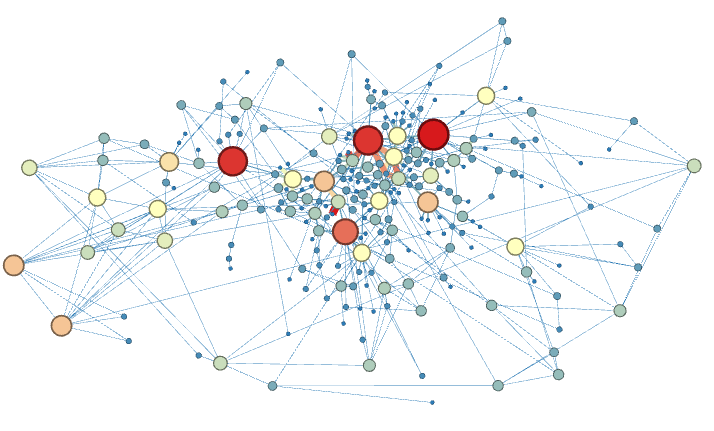
\includegraphics[width=0.5\textwidth]{images/Spain1996q2KK}
        \label{spq2kk}
      }
      \qquad
      \subfigure[Distribución de nodos con Frutcherman \& Reignold.] {
        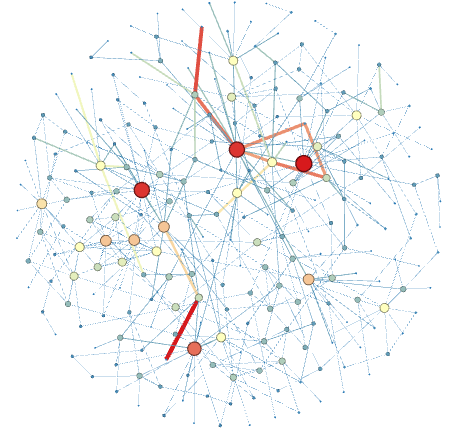
\includegraphics[width=0.35\textwidth]{images/Spain1996q2FR}
        \label{spq2fr}
      }
    }
    \caption{Kamada \& Kawai y Frutcherman \& Reignold para la red Spain-1996 con $q=2$.}
    \label{spq2}
\end{figure}

En la \hyperref[spq2kk]{Figura \ref*{spq2kk}} podemos ver como el algoritmo Kamada \& Kawai hace una distribución ``similar'' a un plano de metro, donde podemos ver de forma más clara, la distribución de la producción científica del país. En los nodos centrales (si el tamaño permitiera ver bien las etiquetas), podemos ver que los nodos más importantes son la medicina y la bioquímica, lléndose hacia la izquierda ramas científicas como la ingeniería, matemática aplicada$\ldots$ Sin embargo, Frutecherman \& Reignold (\hyperref[spq2fr]{Figura \ref*{spq2fr}}) realiza una distribución circular, donde es más difícil interpretar los datos, ya que todos quedan más o menos a la misma distancia, cosa que con Kamada \& Kawai no pasa, ya que aleja los nodos que menos relación tienen entre sí.

\begin{figure}[H]
    \centering
    \mbox {
        \subfigure[Distribución de nodos con Kamada \& Kawai.]{
        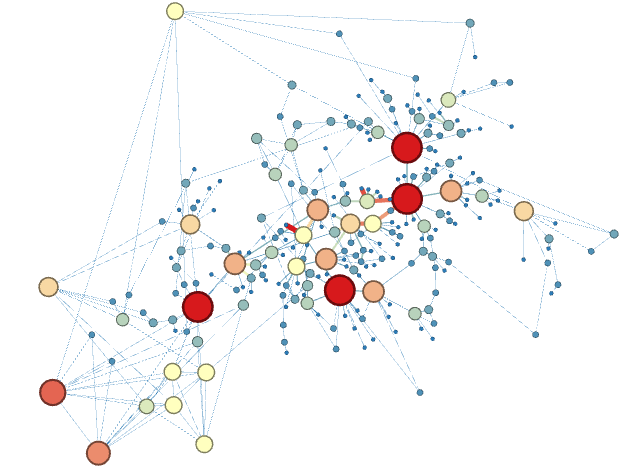
\includegraphics[width=0.5\textwidth]{images/Spain1996q3KK}
        \label{spq3kk}
      }
      \qquad
      \subfigure[Distribución de nodos con Frutcherman \& Reignold.] {
        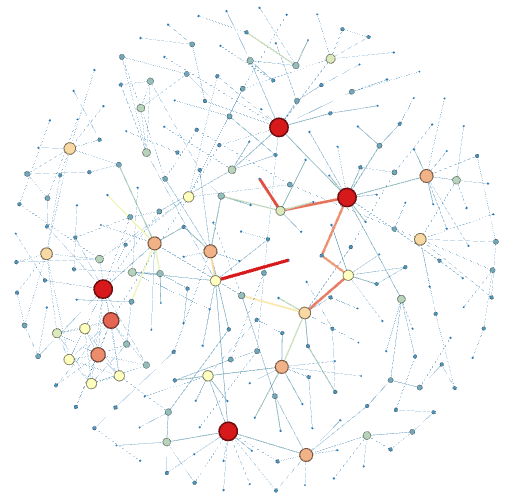
\includegraphics[width=0.35\textwidth]{images/Spain1996q3FR}
        \label{spq3fr}
      }
    }
    \caption{Kamada \& Kawai y Frutcherman \& Reignold para la red Spain-1996 con $q=3$.}
    \label{spq3}
\end{figure}

\begin{figure}[H]
    \centering
    \mbox {
        \subfigure[Distribución de nodos con Kamada \& Kawai.]{
        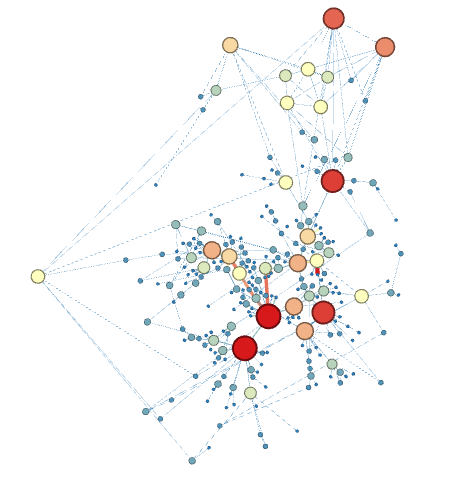
\includegraphics[width=0.35\textwidth]{images/Spain1996q4KK}
        \label{spq4kk}
      }
      \qquad
      \subfigure[Distribución de nodos con Frutcherman \& Reignold.] {
        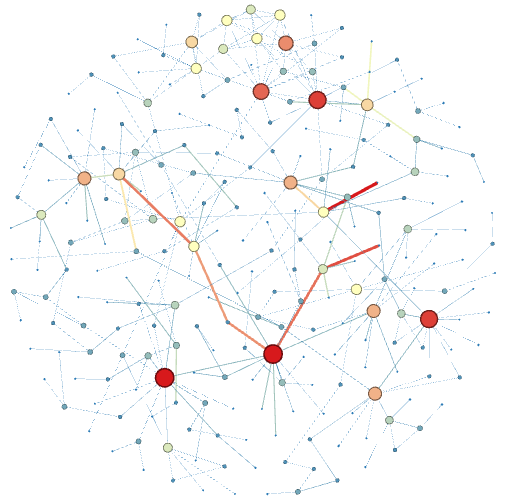
\includegraphics[width=0.35\textwidth]{images/Spain1996q4FR}
        \label{spq4fr}
      }
    }
    \caption{Kamada \& Kawai y Frutcherman \& Reignold para la red Spain-1996 con $q=4$.}
    \label{spq4}
\end{figure}

\begin{figure}[H]
    \centering
    \mbox {
        \subfigure[Distribución de nodos con Kamada \& Kawai.]{
        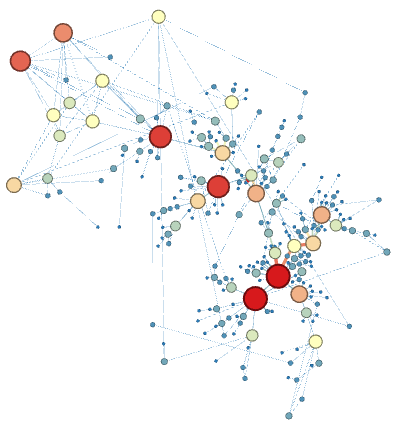
\includegraphics[width=0.35\textwidth]{images/Spain1996qn-1KK}
        \label{spqn-1kk}
      }
      \qquad
      \subfigure[Distribución de nodos con Frutcherman \& Reignold.] {
        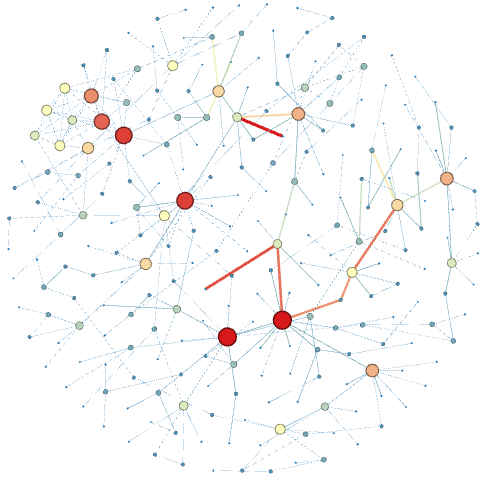
\includegraphics[width=0.35\textwidth]{images/Spain1996qn-1FR}
        \label{spqn-1fr}
      }
    }
    \caption{Kamada \& Kawai y Frutcherman \& Reignold para la red Spain-1996 con $q=n-1$.}
    \label{spqN-1}
\end{figure}

Como se puede ver en cada una de las imágenes podemos ver cómo, para este tipo de red, el algoritmo Kamada \& Kawai realiza una mejor visualización que Frutcherman \& Reignold, dejando más alejadas las materias que no tienen relación entre sí, y más cercanas las que sí tienen relación, mientras que Frutcherman \& Reignold, realiza una visualización circular, al querer dejar los enlaces con la misma longitud.

\subsection{Visualización para la red \textit{Spain-2004.net}}

\begin{figure}[H]
    \centering
    \mbox {
        \subfigure[Distribución de nodos con Kamada \& Kawai.]{
        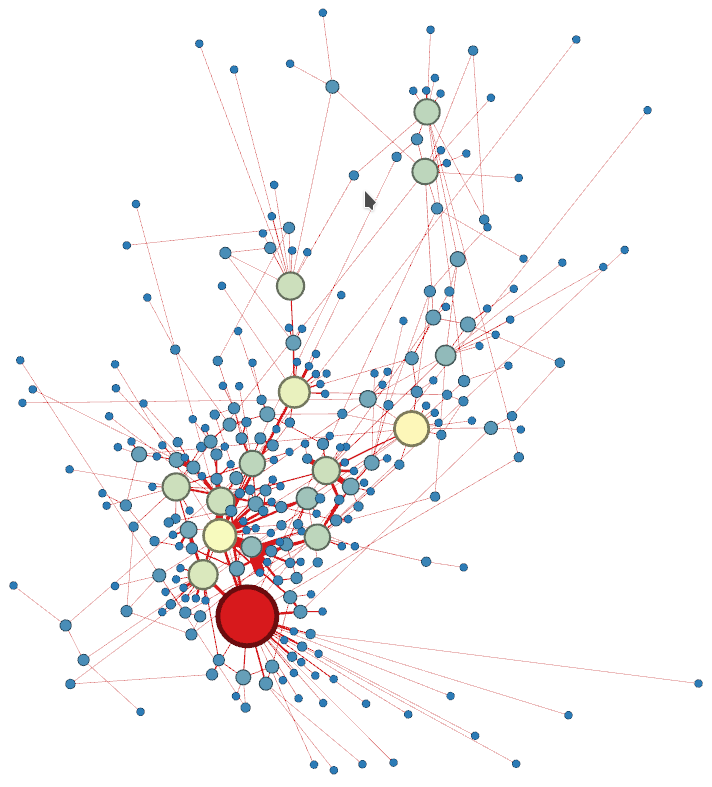
\includegraphics[width=0.4\textwidth]{images/Spain2004q2KK}
        \label{spq2kk04}
      }
      \qquad
      \subfigure[Distribución de nodos con Frutcherman \& Reignold.] {
        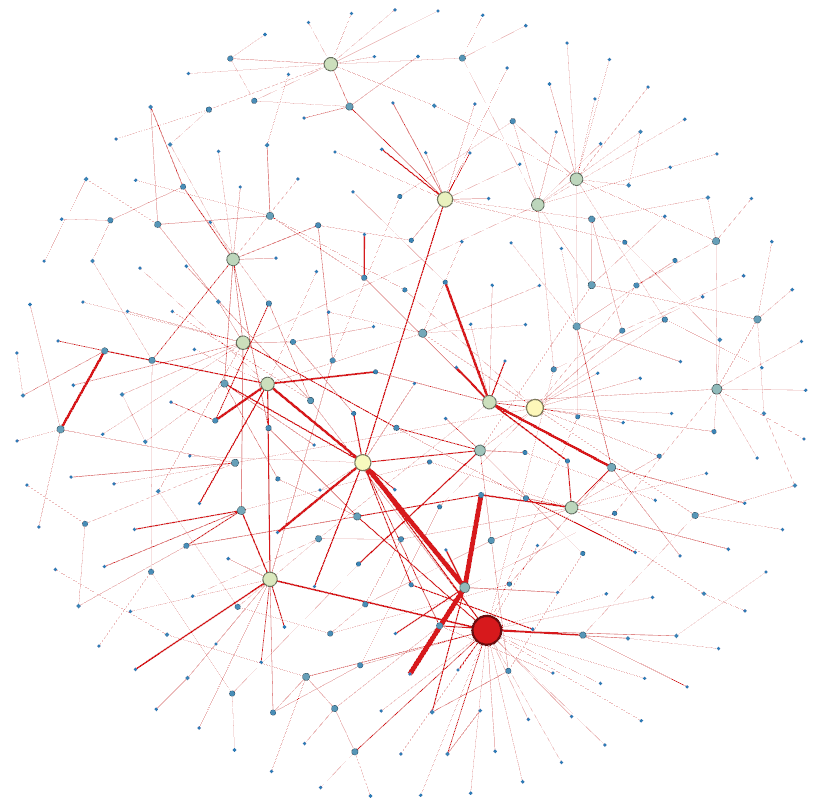
\includegraphics[width=0.4\textwidth]{images/Spain2004q2FR}
        \label{spq2fr04}
      }
    }
    \caption{Kamada \& Kawai y Frutcherman \& Reignold para la red Spain-2004 con $q=2$.}
    \label{spq204}
\end{figure}

En esta red, pasados 8 años desde la anterior, podremos observar la evolución de la producción científica, tomando mucha más fuerza la medicina, y materias como la Neurociencia, la Psicología, Genética, y otros campos relacionados con las Física y la Ingeniería Electrónica, entre otras. Además de esto, en la red original, se ve incrementado casi el doble el número de nodos existentes y un gran aumento en el número de enlaces de la red, observándose cómo aumenta la producción científica de España a lo largo de esos 8 años, a parte de ver cómo van cambiando los principales temas de investigación.

\begin{figure}[H]
    \centering
    \mbox {
        \subfigure[Distribución de nodos con Kamada \& Kawai.]{
        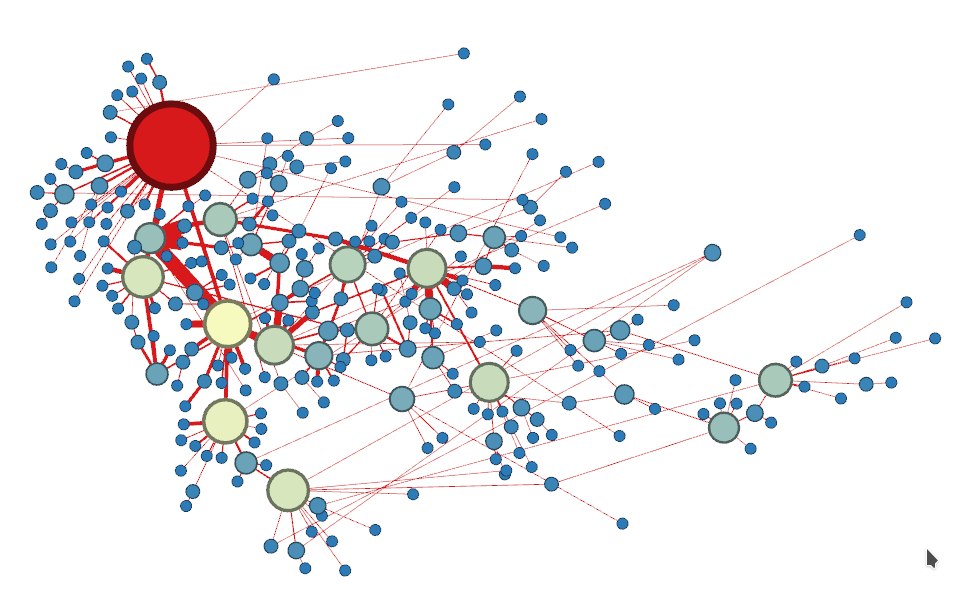
\includegraphics[width=0.5\textwidth]{images/Spain2004q3KK}
        \label{spq3kk04}
      }
      \qquad
      \subfigure[Distribución de nodos con Frutcherman \& Reignold.] {
        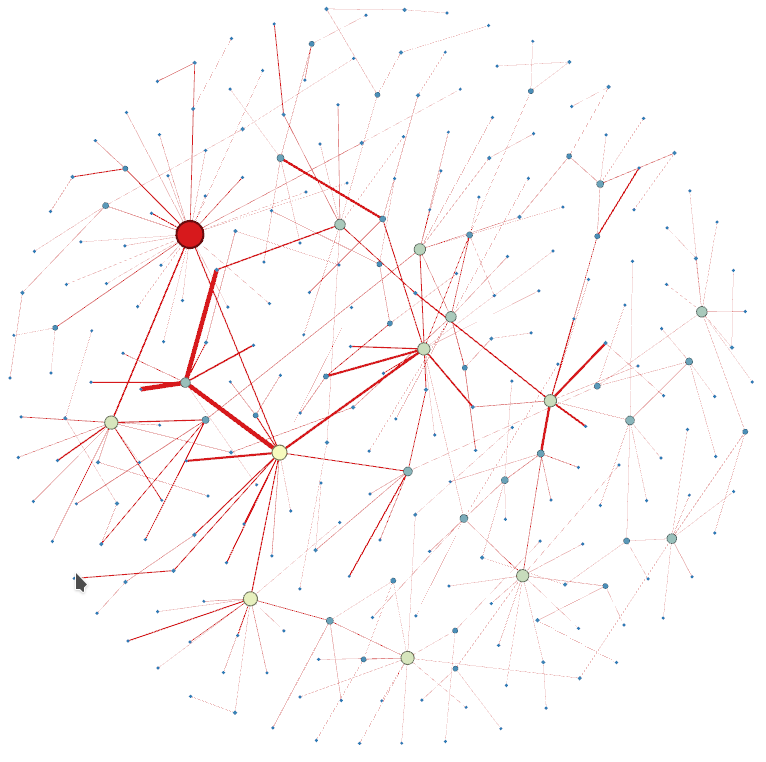
\includegraphics[width=0.35\textwidth]{images/Spain2004q3FR}
        \label{spq3fr04}
      }
    }
    \caption{Kamada \& Kawai y Frutcherman \& Reignold para la red Spain-1996 con $q=3$.}
    \label{spq304}
\end{figure}

\begin{figure}[H]
    \centering
    \mbox {
        \subfigure[Distribución de nodos con Kamada \& Kawai.]{
        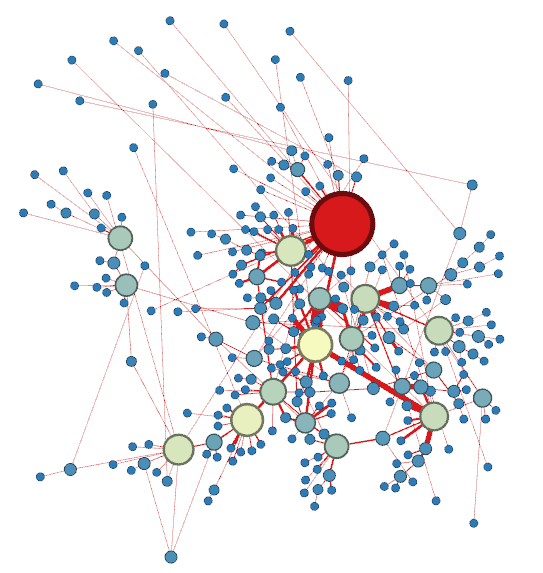
\includegraphics[width=0.35\textwidth]{images/Spain2004q4KK}
        \label{spq4kk04}
      }
      \qquad
      \subfigure[Distribución de nodos con Frutcherman \& Reignold.] {
        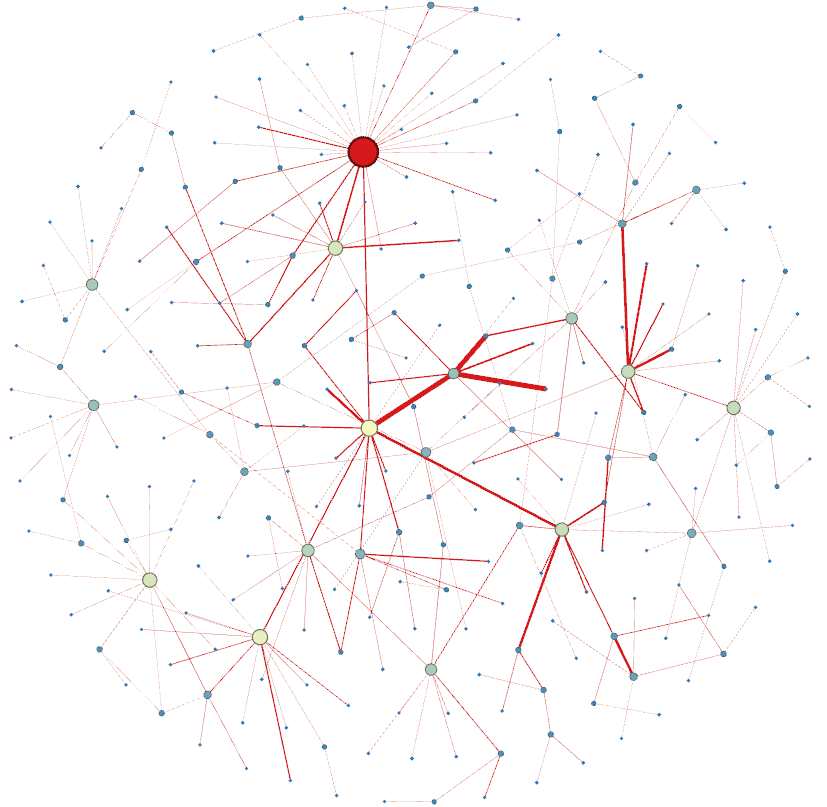
\includegraphics[width=0.35\textwidth]{images/Spain2004q4FR}
        \label{spq4fr04}
      }
    }
    \caption{Kamada \& Kawai y Frutcherman \& Reignold para la red Spain-1996 con $q=4$.}
    \label{spq4}
\end{figure}

\begin{figure}[H]
    \centering
    \mbox {
        \subfigure[Distribución de nodos con Kamada \& Kawai.]{
        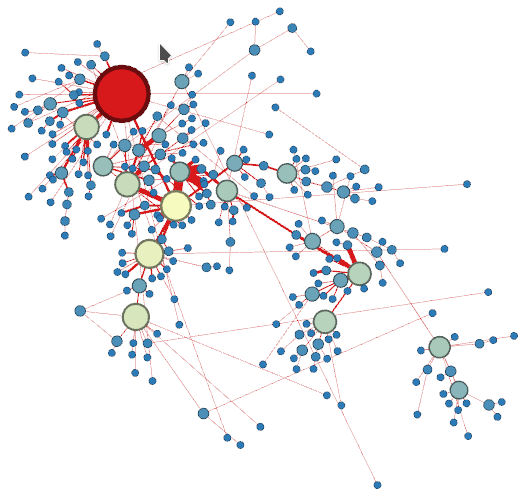
\includegraphics[width=0.35\textwidth]{images/Spain2004qn-1KK}
        \label{spqn-1kk04}
      }
      \qquad
      \subfigure[Distribución de nodos con Frutcherman \& Reignold.] {
        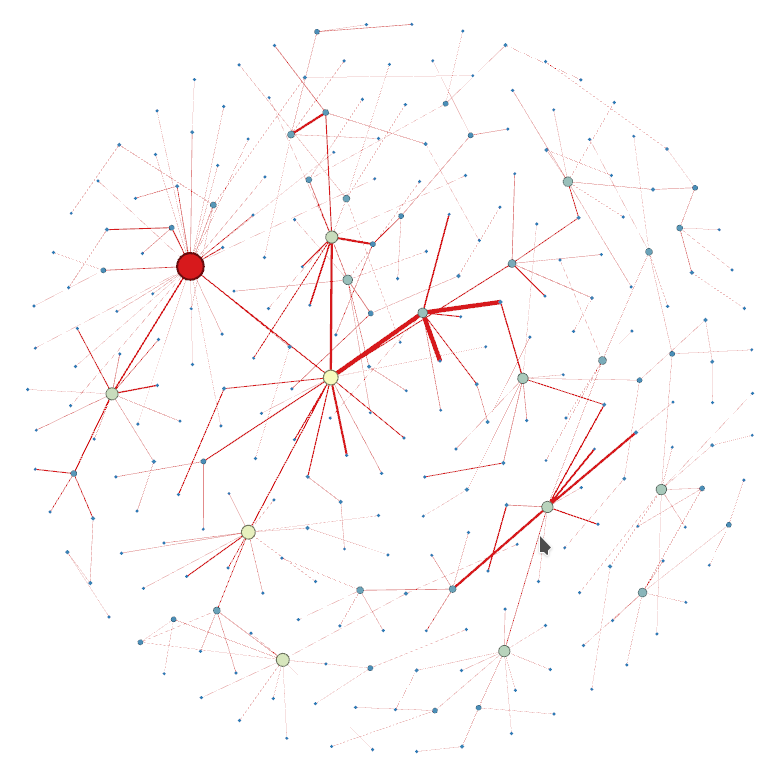
\includegraphics[width=0.35\textwidth]{images/Spain2004qn-1FR}
        \label{spqn-1fr04}
      }
    }
    \caption{Kamada \& Kawai y Frutcherman \& Reignold para la red Spain-1996 con $q=n-1$.}
    \label{spqN-1}
\end{figure}

Al igual que pasaba en la sección anterior, podemos ver que el algoritmo Kamada \& Kawai realiza para este caso una visualización muchísimo mejor que el algoritmo Frutcherman \& Reignold, ya que deja más claro cuáles son los nodos más importantes de la red, realizando esa visualización similar a una línea de metro, mientras que el otro realiza una visualización circular, que para este caso, no deja muy clara la información que transmite la red.


\section{Análisis de eficiencia de las variantes del algoritmo \textit{Pathfinder}}

Para analizar la eficiencia práctica de los distintos algoritmos, vámos a lanzarlos para redes aleatorias de tamaño 500, 1000, 2000, 5000 y 10000 nodos. Para ello, se ha creado un script que ejecuta los algoritmos para las distintas redes y genera una tabla en la que podemos ver los resultados de las distintas ejecuciones.

\begin{table}[H]
\begin{tabular}{cccccccc}
\hline
    $N$ &    $|L|$ &  $|D|$ & Original             & Binary               & Fast                 & MST (Teórico)          & MST (Práctico)         \\
\hline
   500 & 1252 & 0.01003  &   $37.71665$ & $4.40057$  & $0.29051$ & $0.00333$  & $0.00296$ \\
   1000 & 4999 & 0.01000   &  $617.89157$  & $49.98381$ & $2.22931$  & $0.01109$ & $0.01079$ \\
  2000 & 20041 & 0.01002  &  \ensuremath{>} 1800               & $750.72829$  & $18.83852$ & $0.17109$  & $0.10172$  \\
 5000 & 124525 & 0.00996 &  \ensuremath{>} 1800               & \ensuremath{>} 1800               & $276.64002$ & $0.53278$   & $0.48843$   \\
 10000 & 498666 & 0.00997 & \ensuremath{>} 1800               & \ensuremath{>} 1800               & \ensuremath{>} 1800               & $2.53242$    & $2.49397$   \\
\hline
\end{tabular}
\caption{Tabla de resultados para los distintos algoritmos.}
\label{result}
\end{table}


Como se puede ver en la \hyperref[result]{Tabla \ref*{result}}, la versión original del algoritmo Pathfinder, es bastante ineficiente, en comparación con el resto, ya que para problemas de pequeño tamaño, ya requiere una gran cantidad de tiempo y un gran espacio. Esto se debe, al estar basado en programación dinámica, tienen unos ordenes de complejidad en tiempo de $\mathcal{O}(n^4)$ y una complejidad en espacio de $\mathcal{O}(n^3-2\cdot n^2)\equiv\mathcal{O}(n^3)$, que aunque sea polinómica, para problemas donde $n$, ni siquiera es grande, con un $n=1000$ los tiempos de ejecución son del orden de unos 10 minutos en una máquina con un procesador que funciona con \textit{overclock} a $4.6GHz$.

La segunda versión del algoritmo Pathfinder, \textit{BinaryPathfinder}, mejora estos órdenes de complejidad del algoritmo, pero aun así, para problemas de gran tamaño, sigue sufriendo y es incapaz de acabar en tiempos razonables. Esto se debe a que, a pesar de haber rebajado los órdenes de complejidad, estos siguen siendo $\mathcal{O}(n^3\log n)$ para el tiempo, y $\mathcal{O}(4\cdot n^2)$ para el espacio, que aunque sean menores, siguen siendo ``malos'' para problemas donde $n$ es grande.

En la versión \textit{FastPathfinder}, se vuelve a reducir tanto la complejidad en tiempo como en espacio, pasando a tener $\mathcal{O}(n^3)$ para el tiempo, y $\mathcal{O}(3\cdot n^2)$ para el espacio. Esta reducción permite que para problemas donde $n$ es pequeña, pase a tiempos de décimas de segundo, y nos permite ejecutar problemas donde $n = 5000$, en unos 5 minutos aproximadamente. Aun así, a pesar de esta mejora, seguimos poder sin ejecutar problemas donde la $n$ tiene un tamaño medio en un tiempo razonable, es decir, $n > 7000$.

Estas tres versiones utilizan la programación dinámica como algoritmo base, lo que provoca estos órdenes de complejidad tanto en tiempo como en espacio. Las siguientes versiones cambian de paradigma, abandonando la programación dinámica y usando un algoritmo de la teoría clásica de grafos: \textbf{el algoritmo de Kruskal}.

El algoritmo de Kruskal es un algoritmo clásico de la teoría de grafos, muy utilizado para encontrar el árbol generador minimal de un grafo $G$ que toma como entrada, ya que la complejidad en tiempo y espacio es muy pequeña, lo que lo hace muy eficiente. Tomando esto como base, surgieron los siguientes algoritmos.

La versión teórica de esta versión, \textit{MST-Theorical}, es exactamente igual a la versión \textit{MST-Practical} pero cambia la estructura de datos utilizada en los algoritmos. La versión teórica tiene un orden de complejidad menor que la versión práctica, pero los tiempos de ejecución son mayores debido a la estructura de datos que tiene asociada. La versión teórica usa una estructura de datos de conjuntos disjuntos con una unión por rango y comprensión de caminos, mientras que la versión práctica, utiliza una lista indexada de conjuntos disjuntos, es decir, tres listas de enlaces con sus pesos ($F$, $T$ y $H$) junto con el índice. Para más detalle, podemos consultar el artículo original \cite{alg}.

Los órdenes de complejidad son $\mathcal{O}(n^2\cdot\log n)$ para el tiempo y $\mathcal{O}(3\cdot n^2+n)$ para el espacio en la versión teórica del algoritmo MST, mientras que para la versión teórica tenemos $\mathcal{O}(n^3)$ para el tiempo y $\mathcal{O}(3\cdot n^2+n)$ para el espacio. Como podemos ver, la versión teórica tiene unos órdenes de complejidad menor que la versión práctica, pero aun así, gracias a que las estructuras de datos son más simples en la versión práctica, podemos observar en la \hyperref[result]{Tabla \ref*{result}} la versión práctica es más rápida que la teórica.

A pesar de la mejora en tiempo, supone un deterioro en los órdenes de complejidad en espacio, pero es un precio a pagar para poder representar redes con un mayor número de nodos en un tiempo razonable.

\end{document}
